\documentclass[12pt]{article}
\setlength{\oddsidemargin}{0in}
\setlength{\evensidemargin}{0in}
\setlength{\textwidth}{6.5in}
\setlength{\parindent}{0in}
\setlength{\parskip}{\baselineskip}

\usepackage{amsmath,amsfonts,amssymb}
\usepackage{graphicx}
\usepackage{fancyhdr}
\usepackage[]{algorithmicx}
\usepackage{pgfplots}



\pagestyle{fancy}

\begin{document}

\lhead{{\bf CSCI 3104: Algorithms \\ Problem Set 1 (45 points total)} }
\rhead{{\bf Oscar Delgado \\ Summer 2019, CU-Boulder}}
\renewcommand{\headrulewidth}{0.4pt}

\begin{small}
\textit{Advice 1}:\ For every problem in this class, you must justify your answer:\ show how you arrived at it and why it is correct. If there are assumptions you need to make along the way, state those clearly.

\vspace{-3mm}
\textit{Advice 2}:\ Verbal reasoning is typically insufficient for full credit. Instead, write a logical argument, in the style of a mathematical proof.
\vspace{-4mm}
\end{small}

\hrulefill


\begin{enumerate}


	\item\textit{	(5 points) Give an example of an application that uses a proprietary algorithm (i.e. Spotify's "Discover Weekly" playlist, Google's PageRank algorithm, etc.).  Find an article that discusses this algorithm and give a summary of its content.  Provide at least 4-5 sentences for full credit.}

An application the uses Proprietary algorithm is youtube. They use the algorithm is to determine what people want to see. This also has a big affect on the people making the video, such as what the video is about, how long it is, when it was posted, keywords used for the attribute can affect if your video can be successful or not. This is different to their out algorithms before 2012 which recommended based on the highest view count of the video. 2012-2016 then used view duration and session time. Now they use machine learning to filter what you wouldn most likely like and what the average person what like.

citation: https://blog.hootsuite.com/how-the-youtube-algorithm-works/

	\newpage

	% MEDIUM PROBLEM
	\item\textit{ (15 points) Consider two algorithms that perform the same function, that run in  $n/4$ and $log_{2}(n)$, respectively, where $n \in \mathbb{N}$ (i.e. natural numbers). $n$ represents the input size and $n/4$ and $log_{2}(n)$ represent runtimes with respect to the input size.}

	\begin{enumerate}

	\item\textit{ \label{stocks:a} Plot these runtimes on the same graph with the values $n \in [1,50]$ (don't forget labels). Provide the set of intervals over $\mathbb{N}$, where $n/4$ is the strictly better algorithm to use (think greater than, not greater than or equal).}

	\end{enumerate}

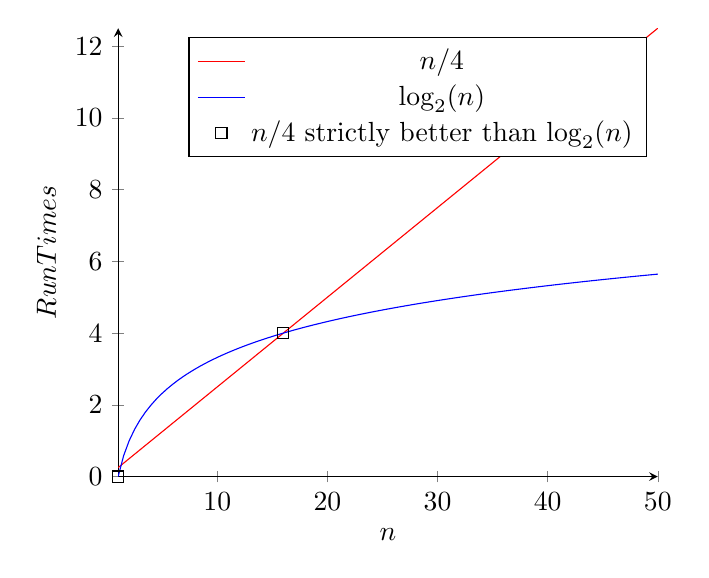
\begin{tikzpicture}
\begin{axis}[
    axis lines = left,
    xlabel = $n$,
    ylabel = {$RunTimes$},
]
%Below the red parabola is defined
\addplot [
    domain=1:50, 
    samples=100, 
    color=red,
]
{x/4};
\addlegendentry{$n/4$}
%Here the blue parabloa is defined
\addplot [
    domain=1:50, 
    samples=100, 
    color=blue,
    ]
    {log2(x)};
\addlegendentry{$\log_2(n)$}

\addplot[
	only marks,
	color=black,
	mark = square,
]
	coordinates{(1,0)(16,4)};
\addlegendentry{$n/4$ strictly better than $\log_2(n)$}

\end{axis}
\end{tikzpicture}

$n/4$ is better than $\log_2(n)$ when $1 < n < 16$. This can be seen in the graph where $n/4$ is lower then $log_2(n)$ and intersect at n=1 and n=16.


	\newpage

	\item \textit{(15 points) Harry the Wizard needs your help solving a riddle deep in an abandoned dwarven mine. There are two doors marked A and B, respectively, and a stone pedestal in the middle of the room inscribed with the following text:}

    \scriptsize

    \textit{"The dwarves who dwelled in  this mine were fond of mathematical drinking games. Two dwarves, Arnold and Barry, are chosen as the participants for this game, and pick functions that they think will best predict the number of people who enter the pub in an hour (\textit{p}) based on the number of drinks they consume in that hour (\textit{d}). They choose $p(d) = d/2$ and $p(d)= 2ln(d)$, respectively. Below is a record of the number of drinks consumed and the corresponding number of patrons patrons who entered the bar over four hours.}

    \begin{center}
        \begin{tabular}{|c | c |}
        \hline
        Number Drinks (\textit{d}) & Number Patrons (\textit{p})\\ \hline
        5 & 4  \\ \hline
        10 & 10  \\ \hline
        15 & 4  \\ \hline
        20 & 8  \\ \hline

        \end{tabular}
    \end{center}

    \textit{Which dwarf, Arnold or Barry, chose the most accurate function?"}

    \normalsize
    \textit{Due to an error in Harry's mental calculations in the last puzzle causing Grog the Barbian to lose his pinky finger, the party demands  a written explanation of the solution to the puzzle. Additionally, since Grog doesn't know how to read, provide a relevant figure in your solution so Grog can believe he is part of the discussion.}

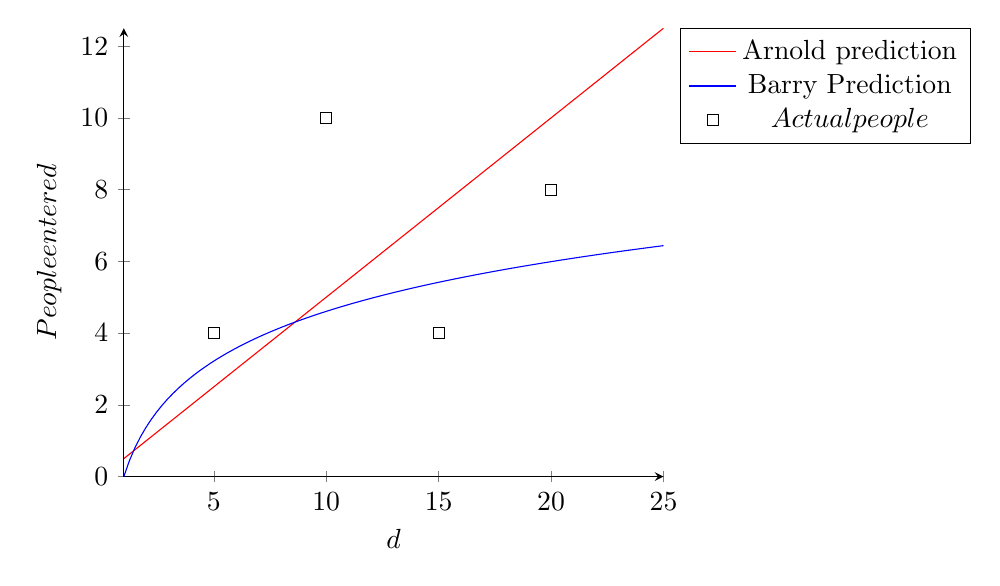
\begin{tikzpicture}
\begin{axis}[
    axis lines = left,
    xlabel = $d$,
    ylabel = {$People entered$},
	legend pos = outer north east
]
%Below the red parabola is defined
\addplot [
    domain=1:25, 
    samples=100, 
    color=red,
]
{x/2};
\addlegendentry{Arnold prediction}
%Here the blue parabloa is defined
\addplot [
    domain=1:25, 
    samples=100, 
    color=blue,
    ]
    {2*ln(x)};
\addlegendentry{Barry Prediction}

\addplot[
	only marks,
	color=black,
	mark = square,
]
	coordinates{(5,4)(10,10)(15,4)(20,8)};
\addlegendentry{$Actual people$}


\end{axis}
\end{tikzpicture}

When examining both cases I determine Barry is more accurate. You can see these in 2 test. First you can visually see 2 of the points (when drinks are 5 and 15) Barry is more accuate and have a tie on d=20. Lastly the most accuate test is by summing all points inaccuacy and adding them together to see who has the lowest score. and Barry win having inaccuacy score of 9.6 and arnold having a score of 12. $(| 4-2ln(5)|+ |10 - 2ln(10)| + |4 - 2ln(15)| + |8 - 2ln(20)| = 9.6$ and did similar step with arnnold and resulting 12)
    \newpage

 	% MEDIUM PROBLEM
 	\item\textit{ (10 points) Consider the following recurrence relation:}
\[
G_n =
     \begin{cases}
       \text{1} &\quad\text{if \textit{n} = 0}\\
       \text{-1} &\quad\text{if \textit{n} = 1}\\
       \text{2} &\quad\text{if \textit{n} = 2}\\
       \text{($G_{n-1}$)($G_{n-2}$)+$G_{n-3}$} &\quad\text{otherwise}\\
     \end{cases}
\]

 	\begin{enumerate}
 	\item\textit{ Write pseudocode for this function that takes in a positive integer, \textit{n}, and returns the \textit{n}th number in the sequence.}

		\begin{verbatim}
	Def G(n) 
	   A = [1,-1,2]
	   For i=3 to n
	      temp = A[2]*A[1]+A[0]
	      A[0] = A[1]
	      A[1] = A[2]
	      A[2] = temp
	   return A[2]
	
	\end{verbatim}
 	\item \textit{What is the 10th number in the sequence?}

	The 10th number in the sequence is: -110655
 	\end{enumerate}


\lhead{ }
\rhead{}
\renewcommand{\headrulewidth}{0pt}

\end{enumerate}

\end{document}
